% ============================================================
%  CHAPITRE 2 — SPÉCIFICATION FONCTIONNELLE ET TECHNIQUE
% ============================================================
\chapter{Spécification Fonctionnelle et Technique}

\chapintro{Ce chapitre formalise les exigences fonctionnelles et non-fonctionnelles
de la plateforme à travers le diagramme de cas d'utilisation global, le diagramme
de classes du domaine, le backlog produit complet et les choix techniques.}

\section{Introduction}

La phase de spécification garantit que l'équipe de développement et les parties
prenantes partagent une vision commune des fonctionnalités à réaliser. Ce chapitre
présente les outils de modélisation utilisés pour formaliser cette vision.

\section{Spécification Fonctionnelle}

\subsection{Exigences Fonctionnelles}

\begin{longtable}{|p{0.8cm}|p{2.8cm}|p{8cm}|}
\caption{Exigences fonctionnelles par rôle}\label{tab:exigences}\\
\hline
\rowcolor{gray!20}
\textbf{N°} & \textbf{Acteur} & \textbf{Exigence} \\
\hline
\endfirsthead
\hline
\rowcolor{gray!20}
\textbf{N°} & \textbf{Acteur} & \textbf{Exigence} \\
\hline
\endhead
\hline
\endlastfoot
EF01 & Tous & S'authentifier avec email et mot de passe (JWT) \\[2pt]\hline
EF02 & Tous & Rafraîchir automatiquement le token d'accès \\[2pt]\hline
EF03 & Tous & Modifier son mot de passe \\[2pt]\hline
EF04 & SuperAdmin & Créer et gérer les tenants (entreprises) \\[2pt]\hline
EF05 & AdminEntreprise & Créer et gérer les garages du tenant \\[2pt]\hline
EF06 & AdminEntreprise & Créer et gérer le personnel (chefs, mécaniciens) \\[2pt]\hline
EF07 & AdminEntreprise & Consulter les indicateurs de performance (KPI) \\[2pt]\hline
EF08 & AdminEntreprise & Enregistrer le paiement d'une intervention \\[2pt]\hline
EF09 & Client & S'inscrire sur la plateforme \\[2pt]\hline
EF10 & Client & Gérer ses véhicules (ajout, consultation) \\[2pt]\hline
EF11 & Client & Soumettre un rapport de symptômes textuels \\[2pt]\hline
EF12 & Système & Générer un diagnostic IA (Ollama RAG) automatiquement \\[2pt]\hline
EF13 & Client & Réserver un rendez-vous dans la plage proposée \\[2pt]\hline
EF14 & Client & Approuver ou refuser un devis \\[2pt]\hline
EF15 & Client & Suivre le cycle de vie de son intervention \\[2pt]\hline
EF16 & Client & Télécharger sa facture en PDF \\[2pt]\hline
EF17 & ChefAtelier & Réviser les rapports et proposer une plage RDV \\[2pt]\hline
EF18 & ChefAtelier & Approuver ou refuser des rendez-vous \\[2pt]\hline
EF19 & ChefAtelier & Assigner des mécaniciens à une tâche de réparation \\[2pt]\hline
EF20 & ChefAtelier & Réviser le rapport d'examen du mécanicien \\[2pt]\hline
EF21 & ChefAtelier & Créer et finaliser une facture (devis) \\[2pt]\hline
EF22 & ChefAtelier & Valider la réparation et notifier le client \\[2pt]\hline
EF23 & Mécanicien & Consulter ses tâches assignées \\[2pt]\hline
EF24 & Mécanicien & Soumettre un rapport d'examen (pièces, observations) \\[2pt]\hline
EF25 & Mécanicien & Soumettre un rapport de fin de réparation \\[2pt]\hline
EF26 & Système & Envoyer notifications in-app (MySQL) et push (FCM) \\[2pt]\hline
EF27 & AdminEntreprise & Gérer l'inventaire des pièces détachées \\[2pt]\hline
EF28 & Tous & Accéder via application Android (client et mécanicien) \\[2pt]\hline
\end{longtable}

% ——————————————————————————————————————————————————————————
\subsection{Diagramme de cas d'utilisation global}

\begin{sidewaysfigure}[p]
\centering
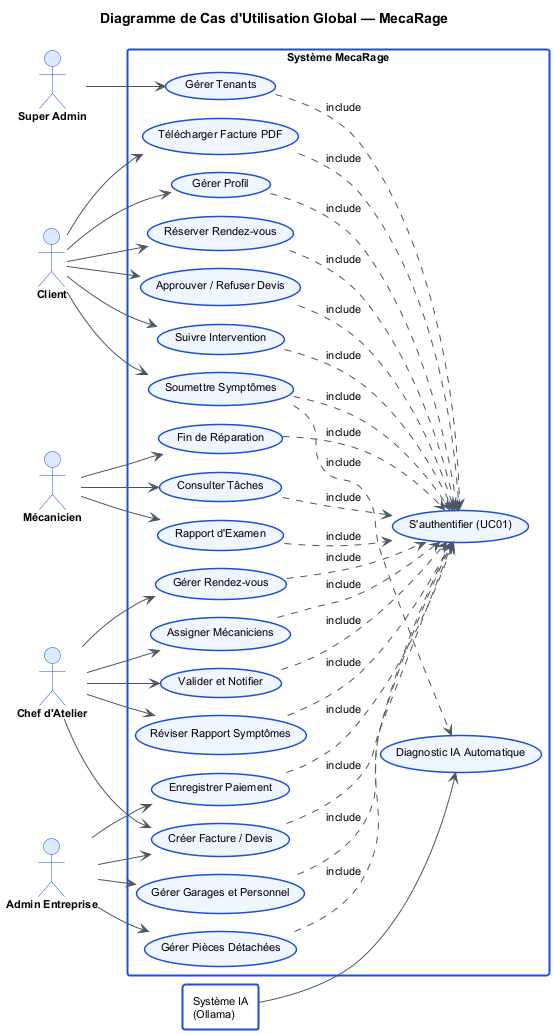
\includegraphics[width=0.92\textheight,height=0.80\textwidth,keepaspectratio]{diagrams/uc_global.png}
\caption{Diagramme de cas d'utilisation global --- MecaRage}
\label{fig:uc-global}
\end{sidewaysfigure}

% ——————————————————————————————————————————————————————————
\subsection{Diagramme de classes global}

\begin{sidewaysfigure}[p]
\centering
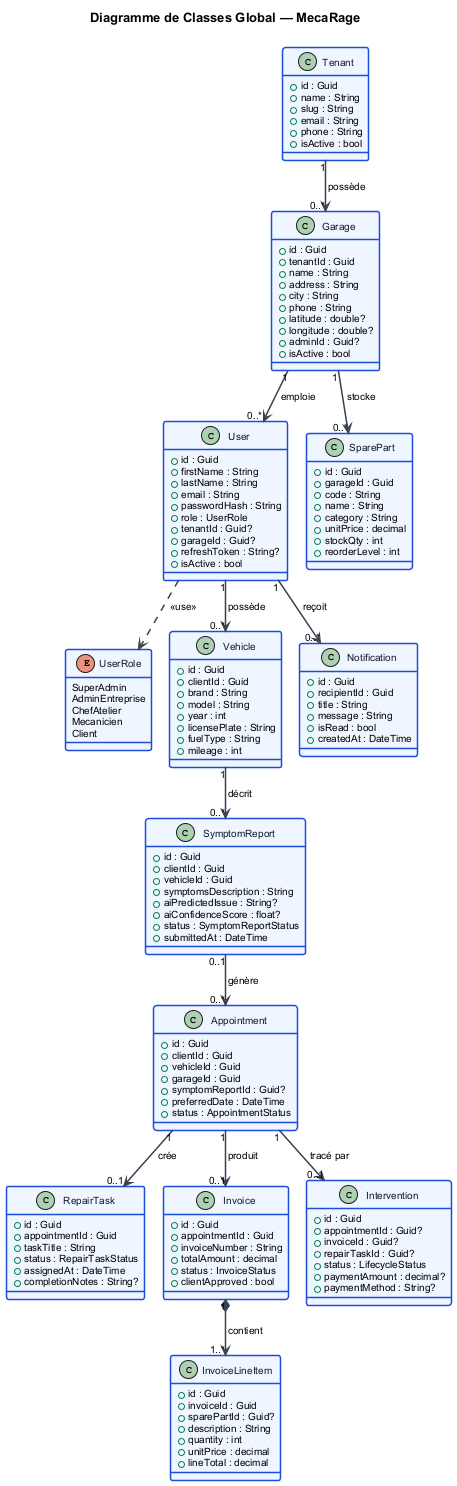
\includegraphics[width=0.92\textheight,height=0.80\textwidth,keepaspectratio]{diagrams/class_global.png}
\caption{Diagramme de classes global --- Entités du domaine MecaRage}
\label{fig:class-global}
\end{sidewaysfigure}

% ——————————————————————————————————————————————————————————
\subsection{Backlog Produit}

\begin{longtable}{|p{0.8cm}|p{2.4cm}|p{5.4cm}|p{1.4cm}|p{0.7cm}|p{1.3cm}|}
\caption{Backlog Produit complet --- MecaRage}\label{tab:backlog}\\
\hline
\rowcolor{gray!20}
\textbf{ID} & \textbf{En tant que} & \textbf{Je veux} & \textbf{Priorité} & \textbf{SP} & \textbf{Sprint} \\
\hline
\endfirsthead
\hline
\rowcolor{gray!20}
\textbf{ID} & \textbf{En tant que} & \textbf{Je veux} & \textbf{Priorité} & \textbf{SP} & \textbf{Sprint} \\
\hline
\endhead
\hline
\endlastfoot
US01 & Utilisateur & M'inscrire avec email et mot de passe & \prio{H} & 3 & Sprint 1 \\[2pt]\hline
US02 & Utilisateur & Me connecter et recevoir un JWT & \prio{H} & 3 & Sprint 1 \\[2pt]\hline
US03 & Utilisateur & Rafraîchir mon token automatiquement & \prio{H} & 2 & Sprint 1 \\[2pt]\hline
US04 & Utilisateur & Modifier mon mot de passe & \prio{M} & 2 & Sprint 1 \\[2pt]\hline
US05 & SuperAdmin & Créer et gérer les tenants & \prio{H} & 3 & Sprint 2 \\[2pt]\hline
US06 & AdminEntreprise & Créer et gérer des garages & \prio{H} & 5 & Sprint 2 \\[2pt]\hline
US07 & AdminEntreprise & Gérer le personnel & \prio{H} & 5 & Sprint 2 \\[2pt]\hline
US08 & Client & Enregistrer et gérer ses véhicules & \prio{H} & 3 & Sprint 2 \\[2pt]\hline
US09 & AdminEntreprise & Gérer l'inventaire des pièces & \prio{M} & 5 & Sprint 2 \\[2pt]\hline
US10 & Client & Soumettre un rapport de symptômes & \prio{H} & 5 & Sprint 3 \\[2pt]\hline
US11 & Système & Générer un diagnostic IA (RAG) & \prio{H} & 8 & Sprint 3 \\[2pt]\hline
US12 & ChefAtelier & Réviser les rapports et proposer une plage RDV & \prio{H} & 5 & Sprint 3 \\[2pt]\hline
US13 & Client & Réserver un rendez-vous & \prio{H} & 3 & Sprint 3 \\[2pt]\hline
US14 & ChefAtelier & Approuver ou refuser un rendez-vous & \prio{H} & 3 & Sprint 3 \\[2pt]\hline
US15 & ChefAtelier & Assigner des mécaniciens à une tâche & \prio{H} & 5 & Sprint 4 \\[2pt]\hline
US16 & Mécanicien & Consulter ses tâches assignées & \prio{H} & 3 & Sprint 4 \\[2pt]\hline
US17 & Mécanicien & Soumettre un rapport d'examen & \prio{H} & 5 & Sprint 4 \\[2pt]\hline
US18 & ChefAtelier & Réviser et valider le rapport d'examen & \prio{H} & 3 & Sprint 4 \\[2pt]\hline
US19 & ChefAtelier & Créer et finaliser une facture & \prio{H} & 5 & Sprint 4 \\[2pt]\hline
US20 & Client & Approuver ou refuser un devis & \prio{H} & 3 & Sprint 4 \\[2pt]\hline
US21 & Mécanicien & Soumettre la fin de réparation & \prio{H} & 3 & Sprint 4 \\[2pt]\hline
US22 & ChefAtelier & Valider et notifier le client & \prio{H} & 3 & Sprint 4 \\[2pt]\hline
US23 & AdminEntreprise & Enregistrer le paiement & \prio{H} & 3 & Sprint 4 \\[2pt]\hline
US24 & Système & Tracer le cycle de vie automatiquement & \prio{H} & 8 & Sprint 4 \\[2pt]\hline
US25 & Utilisateurs & Recevoir notifications in-app et push & \prio{M} & 5 & Sprint 4 \\[2pt]\hline
US26 & Client & Télécharger la facture en PDF & \prio{M} & 3 & Sprint 4 \\[2pt]\hline
US27 & Client/Mécanicien & Utiliser l'application Android native & \prio{M} & 13 & Sprint 4 \\[2pt]\hline
\multicolumn{4}{|r|}{\textbf{Total Story Points}} & \multicolumn{2}{c|}{\textbf{104 SP}} \\
\hline
\end{longtable}

\section{Spécification Technique}

\subsection{Exigences Non-Fonctionnelles}

\begin{table}[H]
\centering
\caption{Exigences non-fonctionnelles}
\label{tab:enf}
\begin{tabularx}{\textwidth}{|l|X|}
\hline
\rowcolor{gray!15}
\textbf{Critère} & \textbf{Exigence} \\
\hline
Performance & Temps de réponse API $<$ 300 ms pour 95\% des requêtes \\[2pt]\hline
Sécurité & JWT HS256, hachage bcrypt, isolation multi-tenant, CORS contrôlé \\[2pt]\hline
Scalabilité & Architecture stateless~; front-end découplé~; services indépendants \\[2pt]\hline
Disponibilité & Docker Compose avec healthchecks et \texttt{restart: unless-stopped} \\[2pt]\hline
Maintenabilité & Clean Architecture, CQRS, tests xUnit, couverture $\geq 70\%$ \\[2pt]\hline
Compatibilité & Android 8+ (API 26)~; navigateurs modernes (Chrome, Firefox, Edge) \\[2pt]\hline
\end{tabularx}
\end{table}

\subsection{Outils et Environnement de Développement}

\begin{table}[H]
\centering
\caption{Stack technologique de MecaRage}
\label{tab:stack}
\begin{tabularx}{\textwidth}{|l|l|X|}
\hline
\rowcolor{gray!15}
\textbf{Couche} & \textbf{Technologie} & \textbf{Version / Rôle} \\
\hline
Front-end Web & Angular + Tailwind CSS & v21.1 / SPA réactive, dark mode \\[2pt]\hline
Back-end API & ASP.NET Core + MediatR & v9.0 / API REST, CQRS, Clean Arch. \\[2pt]\hline
Base de données & MySQL + Pomelo EF Core & 8.0 / ORM relationnel, migrations \\[2pt]\hline
Cache & Redis & 7.0 / sessions, invalidation cache \\[2pt]\hline
Service IA & Python FastAPI + Ollama & 3.13 / RAG BM25 + LLM local \\[2pt]\hline
Mobile & Android Java + Firebase & SDK 26+ / RTDB + FCM \\[2pt]\hline
PDF & QuestPDF & 2026.x / génération factures \\[2pt]\hline
Déploiement & Docker + Docker Compose & 25+ / containerisation totale \\[2pt]\hline
Monitoring & Prometheus + Grafana & --- / métriques et alertes \\[2pt]\hline
Gestion projet & Méthode Agile Scrum & 4 sprints, 2 semaines/sprint \\[2pt]\hline
\end{tabularx}
\end{table}

\section{Conclusion}

Ce chapitre a formalisé les besoins de la plateforme par 27 user stories organisées
en 4 sprints (104 story points au total). Les chapitres suivants détaillent la
conception et le développement de chaque sprint.
